
\documentclass[article,12pt,onesidea,4paper,english,brazil]{abntex2}

\usepackage{lmodern, indentfirst, nomencl, color, graphicx, microtype, lipsum,textcomp}			
\usepackage[T1]{fontenc}		
\usepackage[utf8]{inputenc}		

\setlrmarginsandblock{2cm}{2cm}{*}
\setulmarginsandblock{2cm}{2cm}{*}
\checkandfixthelayout

\setlength{\parindent}{1.3cm}
\setlength{\parskip}{0.2cm}

\SingleSpacing

\begin{document}
	
	\selectlanguage{brazil}
	
	\frenchspacing 
	
	\begin{center}
		\LARGE CONSTRUÇÃO DE JOGOS COMO FERRAMENTA DE ENSINO E APRENDIZAGEM DE MATEMÁTICA APLICADO AO ENSINO TÉCNICO EM FLORESTAS.\footnote{Trabalho realizado dentro da área de Conhecimento CNPq/CAPES: Ciências exatas e da terra com financiamento do Edital de Pesquisa 03 de 2015.}
		
		\normalsize
		Isabella Navarro da Silva\footnote{Bolsista (PIBIC), isabellanavarro7k@gmail.coml, Campus Ji-Paraná.} 
		Letícia Midori Suganuma\footnote{Bolsista (PIBIC), lmidorisuganuma@gmail.com, Campus Ji-Paraná.} 
	Érica Patrícia Navarro\footnote{Orientador(a), erica.navarro@gmail.com, Campus Ji-Paraná.} 
		Andreza Mendonça\footnote{Co-orientador(a), andreza.mendonca@gmail.com, Campus Ji-Paraná.} 
	\end{center}
	
	% resumo em português
	\begin{resumoumacoluna}
	A disciplina de matemática, tradicionalmente, é associada a uma ciência rigorosa, formal e abstrata, essas concepções, muitas vezes são reforçadas por práticas pedagógicas impessoais e, por vezes, sem qualquer associação com a realidade.O grande desafio dos educadores é reverter o ensino dos conteúdos matemáticos de uma forma meramente mecânica em conteúdos significativos para o aluno. Portanto, o objetivo do projeto foi validar jogos com conteúdos de matemática. Foram confeccionados três jogos envolvendo conteúdos de matemática integrados a realidade do curso técnico em florestas. A turma foi avaliada por meio de questões objetivas antes e após aplicação do jogo. A turma foi divida em grupos. Observamos que o resultado obtido foi positivo, os alunos se interessaram e, discutiram sobre o jogo. Os alunos tiveram um maior rendimento nas avaliações após jogarem, visto que a atividade lúdica reforçou o conteúdo teórico ministrado em sala de aula.
		
		\vspace{\onelineskip}
		
		\noindent
		\textbf{Palavras-chave}: Matemática. Interdisciplinaridade. Atividades lúdicas.
	\end{resumoumacoluna}
	
	\section*{Introdução}
	
	A disciplina de Matemática, tradicionalmente, é associada a uma ciência rigorosa, formal e abstrata, essas concepções, muitas vezes são reforçadas por práticas pedagógicas impessoais e, por vezes, sem qualquer associação com a realidade. Dentre os conteúdos que os alunos apresentam dificuldade de aprendizado encontra-se a geometria, aritmética e álgebra.
	
	O saber matemático torna-se cada vez mais necessário no mundo atual, em que se generalizam tecnologias e meios de informação baseados em dados quantitativos e espaciais (OLIVEIRA et al., 2013). É importante destacar que a Matemática deverá ser vista pelo aluno como um conhecimento que pode favorecer o desenvolvimento do seu raciocínio, de sua sensibilidade expressiva, de sua sensibilidade estética e de sua imaginação (BRASIL,1998).
	
	O grande desafio dos educadores é reverter o ensino dos conteúdos matemáticos de uma forma meramente mecânica em conteúdos significativos para o aluno. Surge, então, neste cenário, um recurso muito importante: o jogo. O jogo didático serve para fixação ou treino da aprendizagem. Conforme Smole (2007) além de proporcionar diversão e estar presente na interação com o meio, o jogar desenvolve o espírito construtivo, a imaginação, a capacidade de sistematizar e abstrair e a capacidade de interagir socialmente.
	
	Diante do exposto, o objetivo do projeto foi validar jogos que integrassem conteúdos de matemática aplicados as disciplinas do curso técnico em florestas possibilitando aos alunos do ensino médio aprimorarem os conhecimentos e habilidades matemáticas e o desenvolvimento do raciocínio lógico.
	
	\section*{Material e Método}
	
Foram confeccionados Jogos: Múltiplos de 2 e de 7 e Caça aos Pentágonos com objetivo de fixar os conteúdos sobre múltiplos, aritmética e álgebra, bem como desenvolver o raciocínio lógico dos alunos. Os alunos tiveram aula teórica de matemática sobre o conteúdo do jogo antes de sua aplicação, em seguida aplicada uma avaliação diagnostica. Em seguida, a turma foi divida em quatro grupos. Cada grupo escolheu um membro por rodada para responder uma questão, ganhou a equipe que respondeu o maior número de questões do jogo. Ao final, aplicou-se uma avaliação diagnostica similar a primeira, com objetivo de validar a eficácia do método de ensino.

O trabalho foi realizado com as turmas dos 3° anos (matutino e vespertino) do curso técnico de florestas integrado ao ensino médio do Instituto Federal de Educação, Ciência e Tecnologia de Rondônia (IFRO), Campus Ji-Paraná.
	
	\section*{Resultados e Discussão}
	
Os alunos tiveram aula teórica sobre os conteúdos de matemática aplicados nos jogos, a exemplo do Pentágono (jogo com questões de geometria). A turma foi avaliada por meio de questões objetivas antes e após aplicação do jogo. A turma foi divida em quatro grupos. Cada grupo escolheu um membro por rodada para responder uma questão, ganhou a equipe que completou corretamente o pentágono primeiro (Figura 1).

\begin{figure}[h]
	\centering
	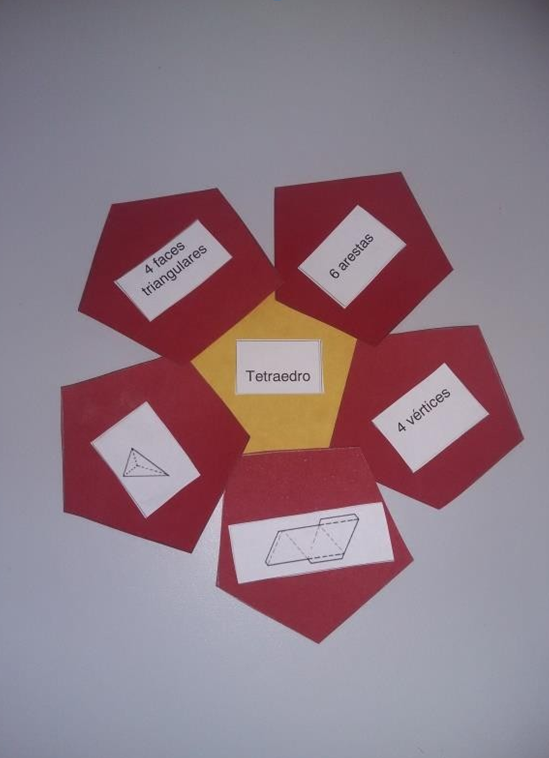
\includegraphics[width=0.35\linewidth]{pip09.png}
\end{figure}

Os alunos avaliaram de maneira positiva o uso do jogo para fixar o conteúdo de geometria, visto que o jogo possibilitou visualizar as figuras bem como fixação das estruturas geométricas. Notou-se que os alunos tiveram um maior rendimento nas avaliações após jogarem, visto que a atividade lúdica reforçou o conteúdo teórico ministrado em sala de aula.

Os alunos conseguiram visualizar as imagens dos poliedros, as diferenças entre vértices, arestas e faces tornando a matemática uma atividade prazerosa e divertida. O uso de jogos para resolver problemas possibilita compreender os argumentos matemáticos e ajuda a vê-los como um conhecimento passível de ser apreendido pelos sujeitos do processo de ensino e aprendizagem (KRULIK, 1997).

Outro exemplo da aplicação dos jogos como ferramenta de ensino foi o jogo múltiplo de 2 e 7 (Figura 2). Notamos que o jogo possibilitou o resgate do conteúdo bem como despertou o raciocínio lógico dos alunos do ensino médio integrado ao técnico. Os resultados corroboram com Oliveira et al (2013) que descrevem que o jogo traz inúmeras contribuições à aprendizagem do aluno, possibilitando o autoconhecimento além de favorecer sua socialização.

\begin{figure}[h]
	\centering
	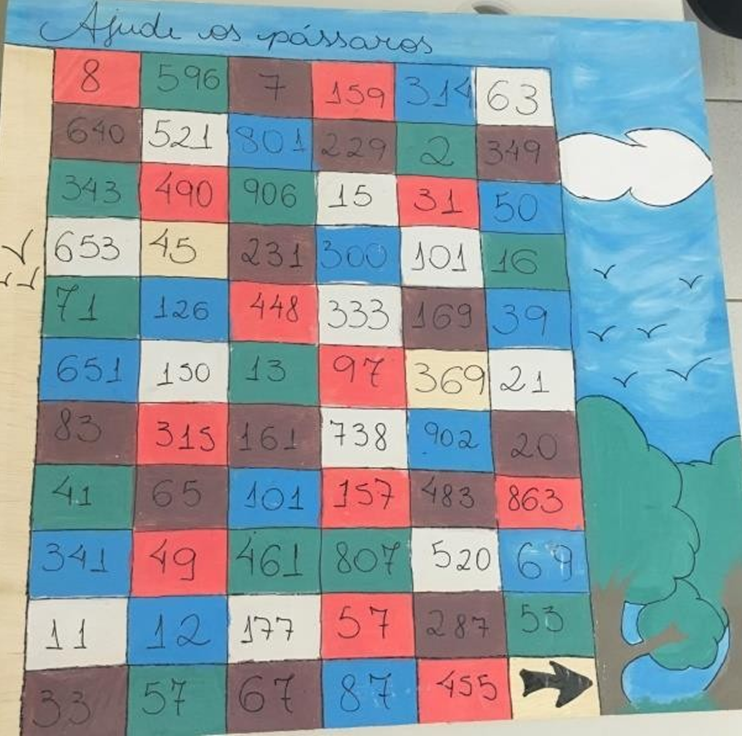
\includegraphics[width=0.35\linewidth]{pip09-2.png}
\end{figure}
	
	\section*{Conclusões}
	
A aplicação de jogos é uma ferramenta facilitadora para o processo de ensino-aprendizagem dos conteúdos de matemática bem como de raciocínio lógico.
O jogo ajudou a visualizar a operação matemática de uma forma mais ampla e dinâmica, fazendo com que haja maior dinamicidade no, processo das operações de multiplicação e divisão, fortalecendo as ferramentas de cálculo mental.
	
	\section*{Instituição de Fomento}
	
	Instituto Federal de Rondônia, Câmpus Ji-Paraná por meio do edital N°03 de 2015, pela concessão das bolsas das duas alunas autoras.
	

	\section*{Referências}
	\sloppy
\noindent BRASIL. Ministério da Educação. Secretaria de Educação Fundamental. Parâmetros Curriculares Nacionais: Matemática. Ensino de 5ª a 8ª Séries e Ensino Médio. Brasília-DF: MEC/SEF, 1998.

\noindent KRULIK, S.; REYS R. E. (orgs) A resolução de problemas na matemática escolar. São Paulo. Atual, 1997.

\noindent OLIVEIRA, D. T. R.; COSTA, E.; TAKAHAMA, S. K. H. A importância dos jogos educativos na aprendizagem da multiplicação com alunos que apresentam deficiência intelectual e cursam a 5ª série do colégio estadual Vítor Soares. Revista EXITUS. V. 03, N°02.p.123-135. 2013.

\noindent SMOLE, Katia C.S; DINIZ, Maria Ignez; CANDIDO,Patrícia. Cadernos doMathema:Jogos de Matemática de 1º ao 5º ano – Ensino Fundamental. Porto Alegre:Artmed, 2007.

\noindent FUCKS, W. R. Matemática Moderna. São Paulo: Polígon, 1970.

\noindent TASHIMA, M. M e SILVA, A. L. da. As lacunas no ensino-aprendizagem da geometria. Universidade Estadual de Londrina. \url{https://www.researchgate.net/publication/238757213\_As\_Lacunas\_No\_Ensino-Aprendizagem\_Da\_Geometria}
	
\end{document}